% Answer to the opening hook: in Adelson's checker shadow, squares A and B are the same grey (#6F6F6F
% in the image). Slide 2 joins them with a band of exactly that grey. Band corners were measured on a
% 700 px render of the image (A centre at 52% / 69%, B centre at 51% / 46%, from bottom left).
\begin{tikzpicture}
  \node[anchor=south west, inner sep=0] (im) at (0,0) {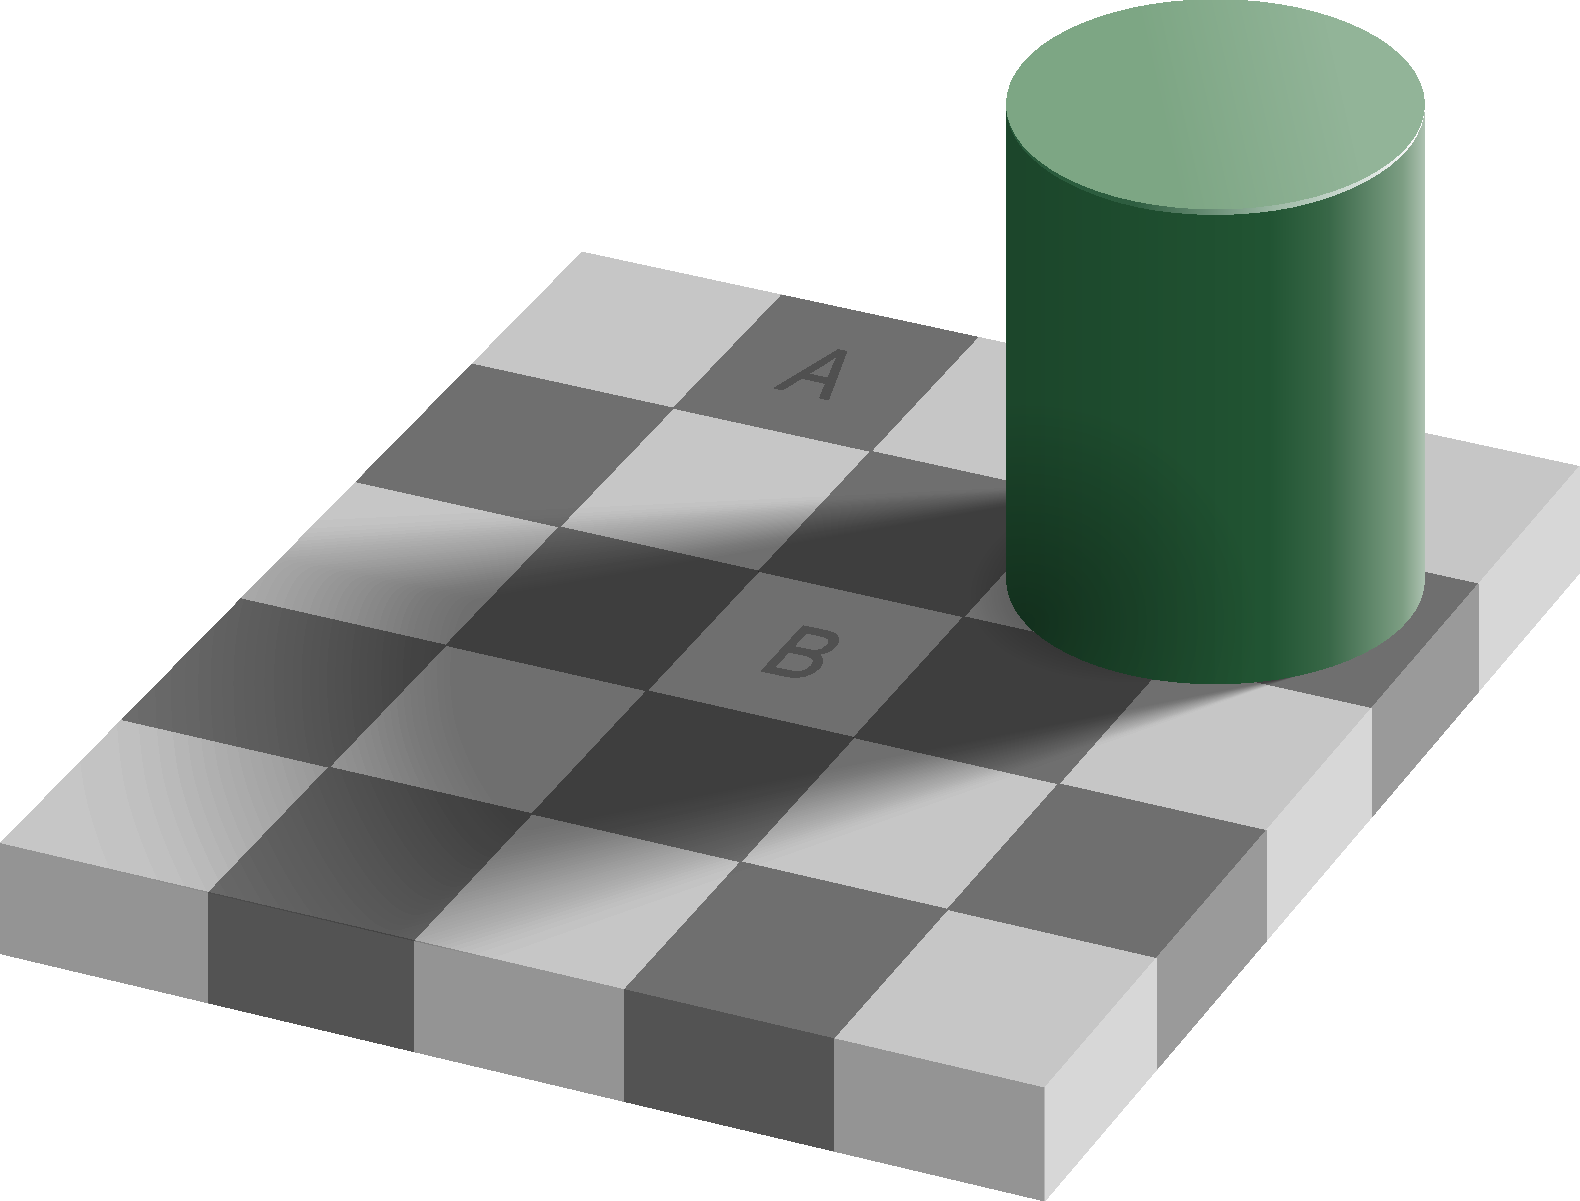
\includegraphics[width=7.4cm]{checker_shadow.pdf}};
  \begin{scope}[x={(im.south east)}, y={(im.north west)}, visible on=<2->]
    \fill[checkgray] (0.499,0.69) -- (0.547,0.69) -- (0.534,0.456) -- (0.486,0.456) -- cycle;
  \end{scope}
\end{tikzpicture}
